\chapter{設計}
\label{implementation}

本章では提案手法の実装について述べる.

\section{本システムのアーキテクチャ}
提案システムにおいて1人の演奏者の演奏から相手の演奏者のスピーカーから音が出るまでをたどると\ref{fig:architecture}のような形になる.

\begin{figure}[htbp]
  \centering
  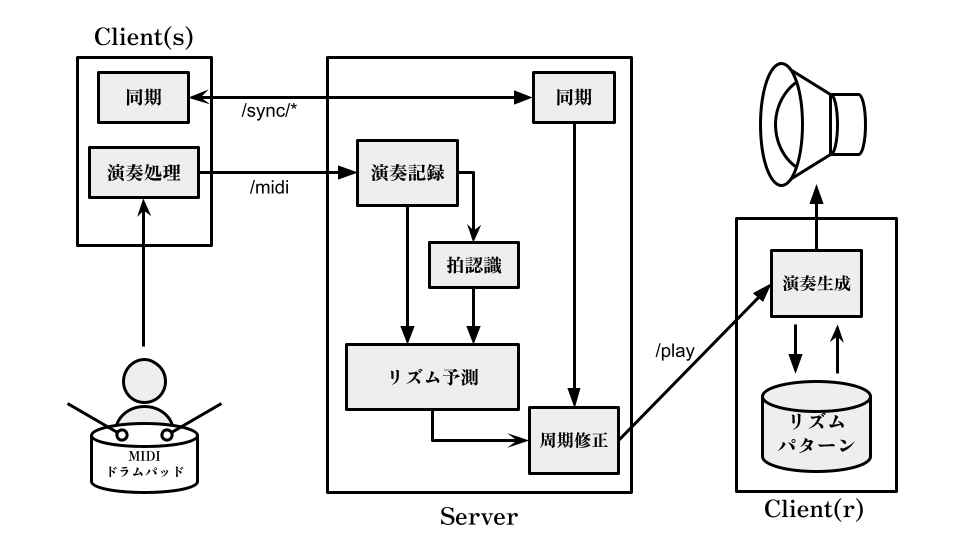
\includegraphics[width=0.8\linewidth]{src/img/architecture.png}
  \caption{本システムのアーキテクチャ}
  \label{fig:architecture}
\end{figure}

演奏がMIDI形式で処理され,サーバーに送信されると演奏履歴に保存される.
頻繁にに演奏履歴に基づいて拍認識が行われて,その情報を元にリズム予測を行なう.
予測したリズムパターンのインデックスをクライアントに送信し,それを受け取ったクライアントは演奏の合成を行ない,予測した演奏が再生される.

サーバ―クライアント間のコミュニケーションはすべてOSCで行っていて,それぞれのOSCアドレスは矢印の下に表記されてある.

「同期」は1秒に一度クロックの誤差,遅延の大きさの2つを測定するためにあるプロセスである.

\section{演奏情報の表現}
本研究では演奏をMIDIの形式であらわし,演奏情報を伝達する.
MIDIは主に物理的なコネクタを通した通信を前提とした楽器制御情報,演奏情報を電子機器間で伝達するためのプロトコルである.\cite{midi}
MIDIキーボード,MIDIドラムパッドなどMIDIをリアルタイムで扱う様々な電子楽器も存在していて広く普及している.

\begin{figure}[htbp]
  \centering
  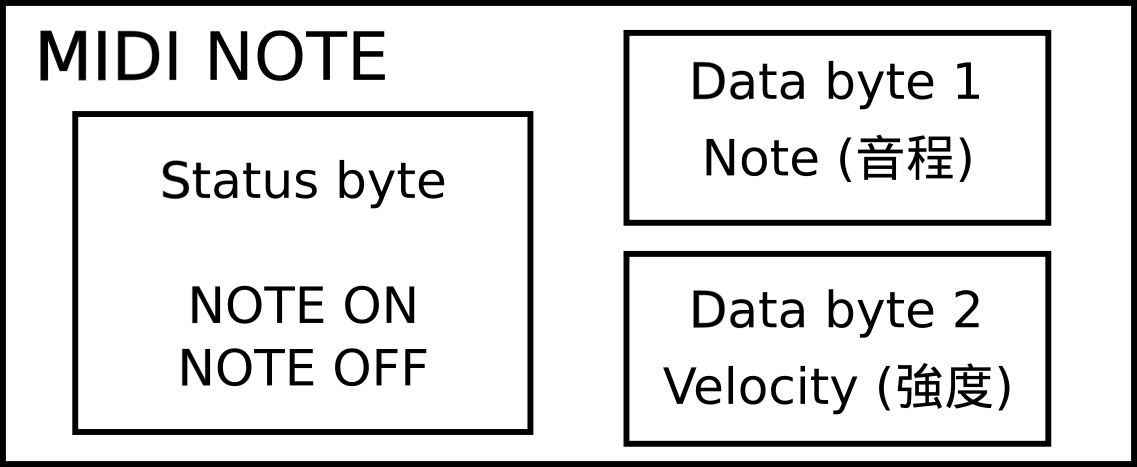
\includegraphics[width=0.8\linewidth]{src/img/midi_spec.png}
  \caption{MIDIメッセージ\cite{midi}}
  \label{fig:midi}
\end{figure}

本研究で扱うMIDIメッセージは最もシンプルな形で,3つのバイトから成り立つ.
Status byteは主に音を始める瞬間,止める瞬間を制御する.
Data byteは2つあり,一つは音程を扱い,もう一つは強度,音の大きさや激しさを制御する.

\section{Open Sound Control}
Open Sound Control (OSC)\cite{opensoundcontrol}はソフトやコンピュータ同士でリアルタイムの通信を行うためのプロトコルである.
元々ネットワークを経由した楽器の演奏を前提として開発されているためデータ型としてMIDIを使えるうえ,時刻タグ(OSC Time Tag)をメッセージとまとめて送ることで正確な音の再生のタイミングを送信者から指定することが可能である.
そのうえ,OSCは広く使われていてライブラリや実装が豊富であるため本研究のシステムで採用した.

\begin{figure}[htbp]
  \centering
  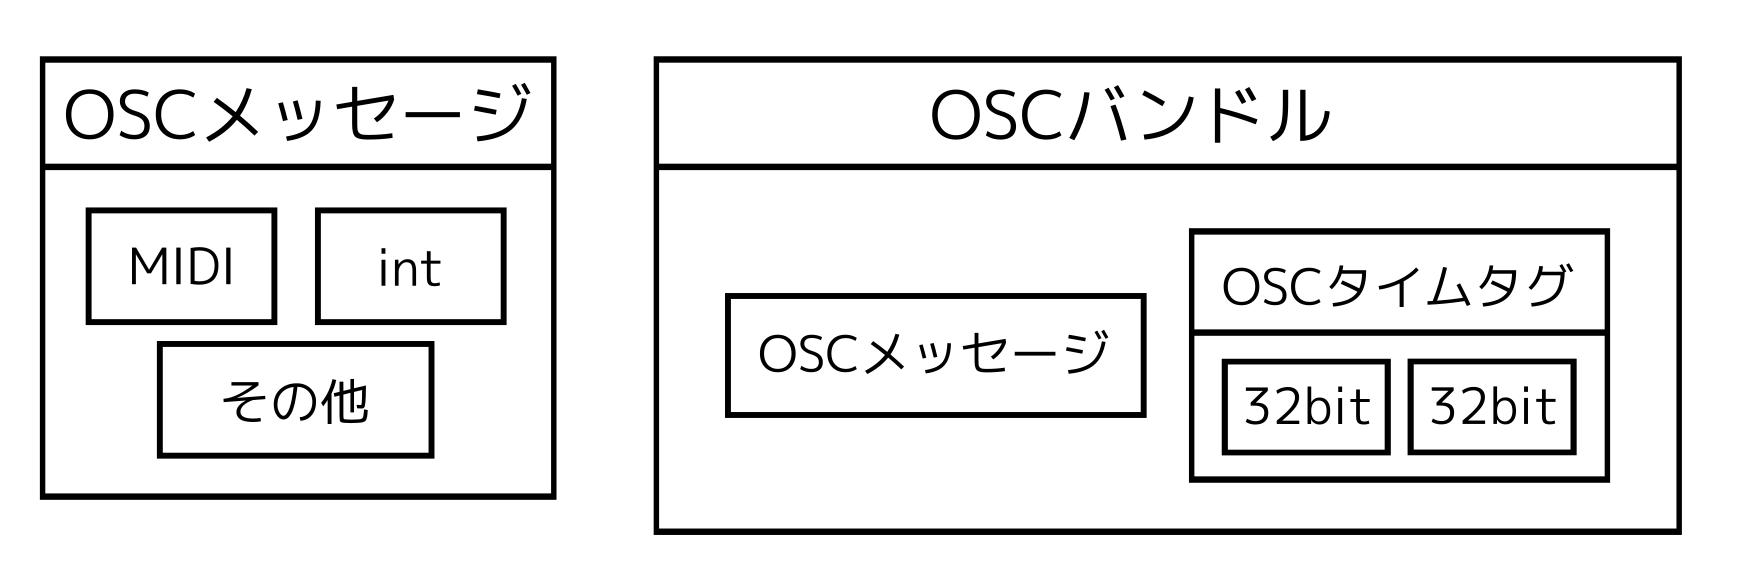
\includegraphics[width=0.8\linewidth]{src/img/g1736.png}
  \caption{OSCメッセージとOSCバンドル}
  \label{fig:oscmess}
\end{figure}

OSCのメッセージは単体で,もしくは時刻を指定して同時に再生する複数のメッセージをバンドルにまとめて送ることができる.
32ビットでUNIX時間での秒数を,32ビットで秒数の小数部を表す時刻タグをOSCで使用されるため高解像度で再生の管理が可能であり,時刻タグの精度は本研究では十分とする.

OSCサーバーがOSCメッセージやOSCバンドルを受信するとそれらを引数としてOSCメソッドが実行される.
OSCメソッドはOSCアドレス空間というツリー構造の中に配置され,OSCメッセージやOSCバンドルに付属されるOSCアドレスを宛先として実行されるOSCメソッドが選ばれる.

\section{拍認識の実装}
演奏予測を行い,相手の演奏を再生するためには2人の演奏のテンポを知る必要がある.
人間的な誤差,または表現の一環として楽曲を通して演奏のテンポは変化していくため,リアルタイムで直近数秒間の演奏を参照して現在のテンポを認識するアルゴリズムが必要である.
本システムの拍認識では\cite{dixon:2000}で使われたアルゴリズムを用いる.

この拍認識アルゴリズムではDixonのアルゴリズム\cite{dixon}に従って打鍵間隔(Inter-onset interval: IOI)のクラスタリングを行う.
IOIとは任意の2つの音の開始時点の時間間隔のことを指す.
このアルゴリズムの分脈では0.025秒から2.5秒の間のIOIしか扱わず,これより小さいIOIは「同時に鳴った音」として扱う.
ある演奏区間に存在するすべての有効なIOIに対し以下のようにクラスタリングを行う.

\begin{algorithm}
  \caption{Dixon's IOI Clustering Algorithm}
\begin{algorithmic}[1]
\For{each pair of onset times \( t_i, t_j \) with \( t_i < t_j \)}
    \If{\( 0.025 < t_j - t_i < 2.5 \)}
        \State Let \( I = t_j - t_i \)
        \State Find cluster \( C_k \) such that \( | Average ( C_k ) - I | \) is minimum
        \If{\( k \) exists and \( | Average(C_k) - I | < \Delta \)}
            \State \( C_k \gets C_k \cup \{ I \} \)
        \Else
            \State Create new cluster \( C_m := \{ I \} \)
        \EndIf
    \EndIf
\EndFor
\end{algorithmic}
\end{algorithm}

このアルゴリズムでは全クラスタのうち,平均値が最も近いクラスタに対して,その平均値との差が\(\Delta\)以下の場合にのみIOIをクラスタに追加する.
クラスタリングの結果もっとも頻度が高いIOI: \begin{math}IOI_f\end{math}を算出したら,その区間のBPMは \begin{math}IOI_f/60\end{math}と推定できる.
この計算は現代のコンピュータでは1秒もかからずに終わり,リアルタイムで拍認識を行なうことが可能なのでこのアルゴリズムを採用した.

\subsection{共通テンポの算出}
複数人を含めた音楽演奏の場合かならず各演奏者の演奏してるテンポはすこしずつずれている.
ネットワーク音楽演奏システムでは演奏者にとって最も演奏がしやすい方式でテンポの合意をとる必要がある.
楽器の発話,リーダーフォロワー構造などの状況に応じてこれに様々なアルゴリズムを用いることができるが,本研究では単純に\ref{commontempo}のように二人の演奏者間の中央値を共通のテンポと認識することとした.

\begin{displaymath}
  BPM_{new} = \frac{BPM_a + BPM_b}{2}
\label{commontempo}
\end{displaymath}

\section{演奏予測の実装}
\ref{prediction}でも記述した通り演奏予測には様々な手法があり,今後益々精度があがり様々な音楽ジャンルに対応できるようになるものと考える.

今回は音楽的な表現の伝達に十分な精度しか必要ないため,簡易的でリアルタイムで処理ができることを優先して\cite{tablanet}で用いられた予測システムを参考に作成した.

\begin{figure}[htbp]
  \centering
  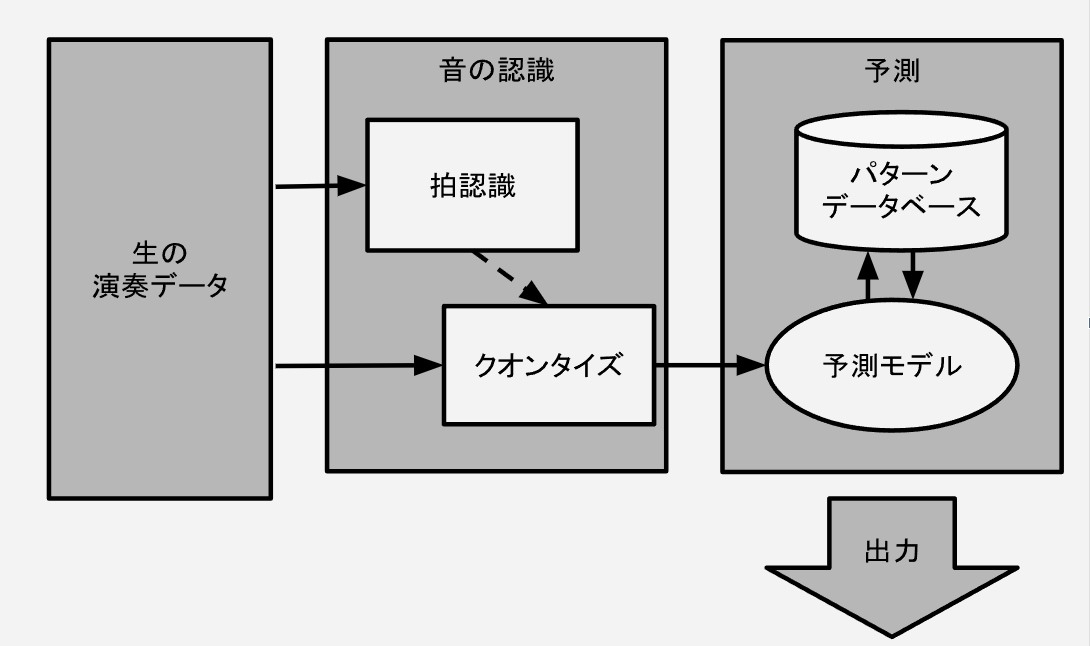
\includegraphics[width=0.8\linewidth]{src/pred.png}
  \caption{予測システム}
  \label{fig:tablenet}
\end{figure}

事前に数十個のリズムパターンを用意し,パターンデータベースとした.
これらのリズムパターンはいずれも1小節のものを作成した.

演奏履歴から直近の16音をとり,それらの音のデルタ時間を入力としてパターンデータベースから次に来るリズムパターンのインデックスを出力するRNNモデルを作成し,本システムに用いた.
学習には事前に行った模擬演奏を用いた.

\subsection{クロック同期,遅延測定}
OSCタイムタグはUNIX時間を基準にした絶対的な時間で送られるため,各クライアントのわずかな時計のずれで再生時間が変わってしまう.
そのため時計のずれを考慮したタイムタグの修正が必要である.
本システムでは簡易的であり,十分な精度が得られるという理由でCristianのアルゴリズム\cite{cristian}を採用している.

\ref{fig:architecture}で示されている通りこの同期を行なうためのプロセスは常に1秒毎に行われている.

\begin{figure}[htbp]
  \centering
  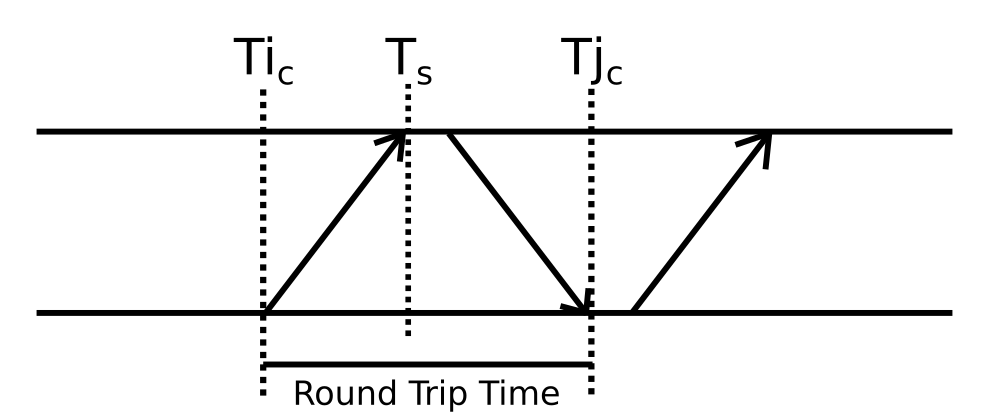
\includegraphics[width=0.8\linewidth]{src/img/cristian.png}
  \caption{本システムのCristianアルゴリズム}
  \label{fig:cristian}
\end{figure}

まずクライアントがサーバー宛に/sync/pingに空のメッセージを送る.
このときクライアントはメッセージを送信した時間\begin{math}
  Ti_c
\end{math}を記録している.
サーバーがこのメッセージを受け取るとサーバー時間\begin{math}
  T_s
\end{math}
を含んだメッセージを即座にクライアント宛に/sync/pongに送信する.
最後にクライアントがこれを受取り,/sync/pongのメッセージを受け取った際のクライアント時間\begin{math}
  Tj_c
\end{math}
を用いて以下の計算で遅延 (latency)とサーバー時間との差 (offset)を算出する.
\begin{displaymath}
  latency_c = \frac{RTT}{2} = \frac{Tj_c - Ti_c}{2}
\end{displaymath}
\begin{displaymath}
  offset_c = Tj_c - (T_s + latency)
\end{displaymath}
RTT (Round Trip Time)は往復にかかった時間であり,ネットワークのレイテンシー,OSCの処理を含めて片方からもう片方へ信号が届くまでの2倍の時間と考える.
最後にこれらの計算結果をサーバーに/sync/recを通して送り返している.

サーバー側ではこれらの計算結果を記録し,メッセージを送る際にはタイムタグ
\begin{displaymath}timetag_c = timetag_s + offset_c\end{displaymath}
として送っている.

%%% Local Variables:
%%% mode: japanese-latex
%%% TeX-master: "../bthesis"
%%% End:
